\chapter{Result}
Now we can use our method to determine $dS/dt$, $Pre$, $ET$ and $R$. After that, we can combine these results and discuss the trend of water storage in Ob basin and the reason for it.
\section{Equivalent water height}
As mentioned in chapter 4, we used 3 methods to calculate the time series of the equivalent water height with the data from CSR, in \ref{fig:TWSA3} we can see 3 curves fit others well. 
\begin{figure}[htbp]
	\centering
	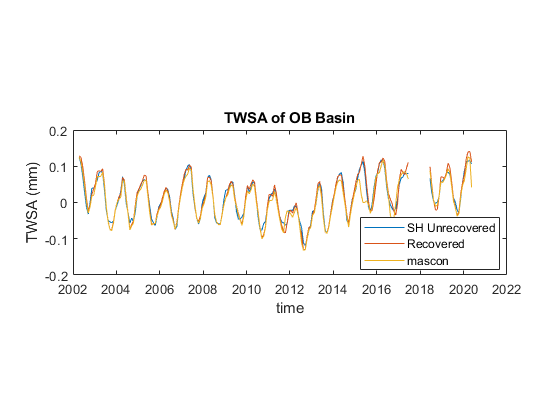
\includegraphics[width=0.7\textwidth]{TWSA3} % Datei in "bilder/" bei LaTeX: eps, bei PDFLaTeX: jpg (o.ä.) 
	\caption{equivalent water height using 3 methods} 
	\label{fig:TWSA3}
\end{figure}
Thus, we can use the spherical harmonic methods(unrecovered) to get all the equivalent water height for all data centers without doubt. see figure(\ref{fig:twsa})
\begin{figure}[htbp] \label{fig:twsa}
	\centering
	\begin{minipage}[t]{0.45\textwidth}
		\centering
		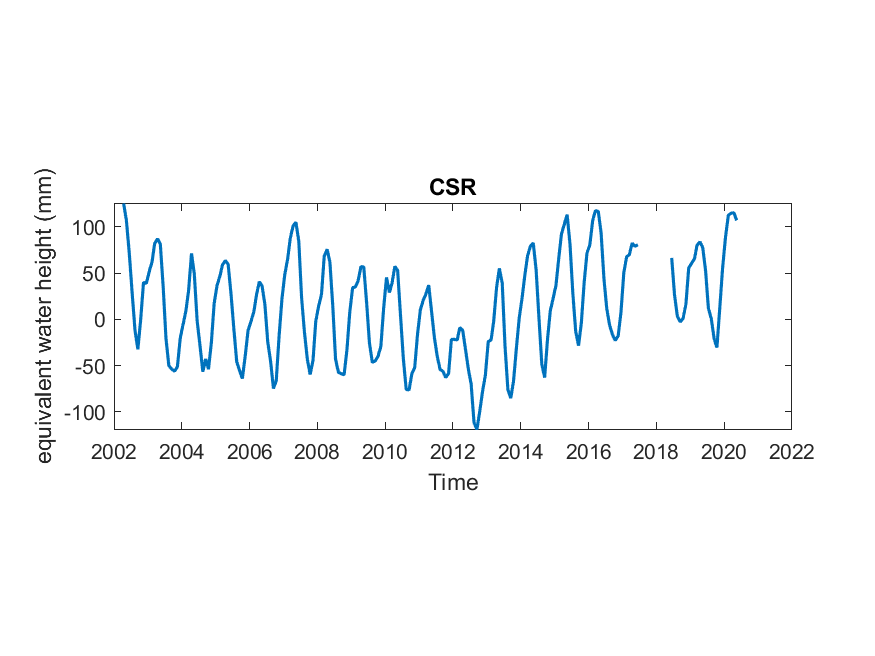
\includegraphics[width=0.8\textwidth]{CSR_TWSA} % Datei in "bilder/" bei LaTeX: eps, bei PDFLaTeX: jpg (o.ä.) 
		\label{fig:CSR}
	\end{minipage}
	\begin{minipage}[t]{0.45\textwidth}
		\centering
		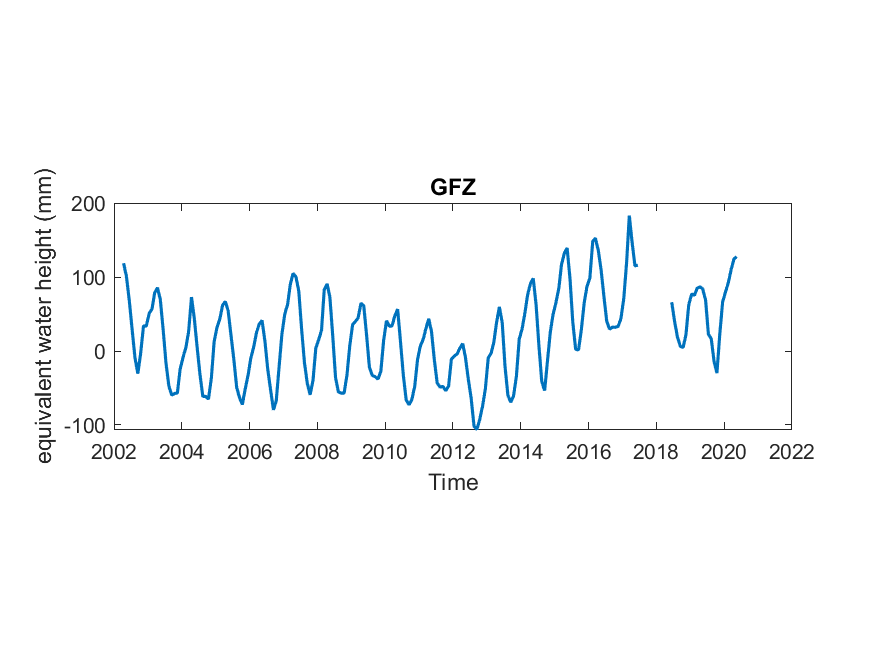
\includegraphics[width=0.8\textwidth]{GFZ_TWSA} % Datei in "bilder/" bei LaTeX: eps, bei PDFLaTeX: jpg (o.ä.) 
		\label{fig:GFZ}
	\end{minipage}
	\begin{minipage}[t]{0.45\textwidth}
		\centering
		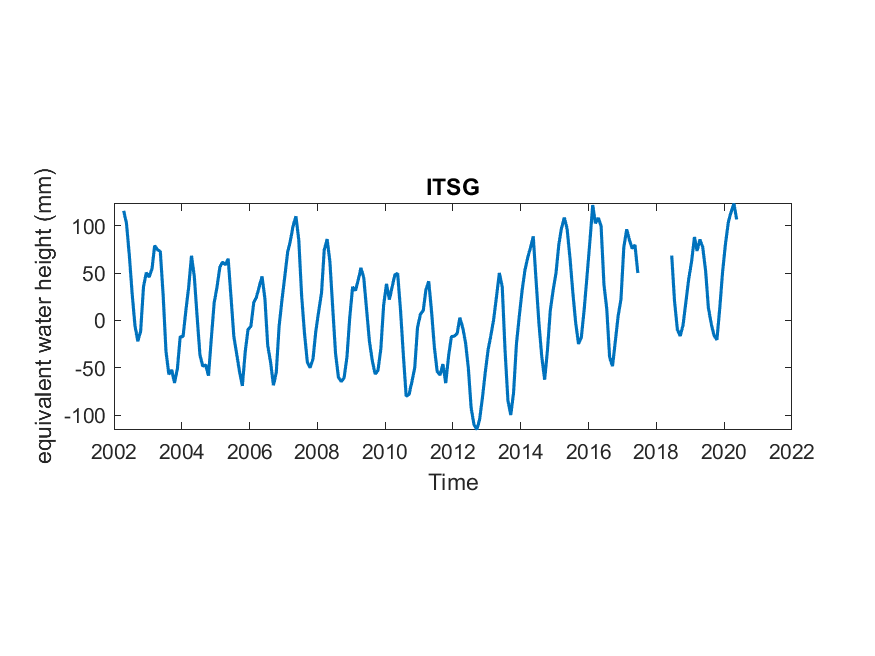
\includegraphics[width=0.8\textwidth]{ITSG_TWSA} % Datei in "bilder/" bei LaTeX: eps, bei PDFLaTeX: jpg (o.ä.) 
		\label{fig:ITSG}
	\end{minipage}
	\begin{minipage}[t]{0.45\textwidth}
		\centering
		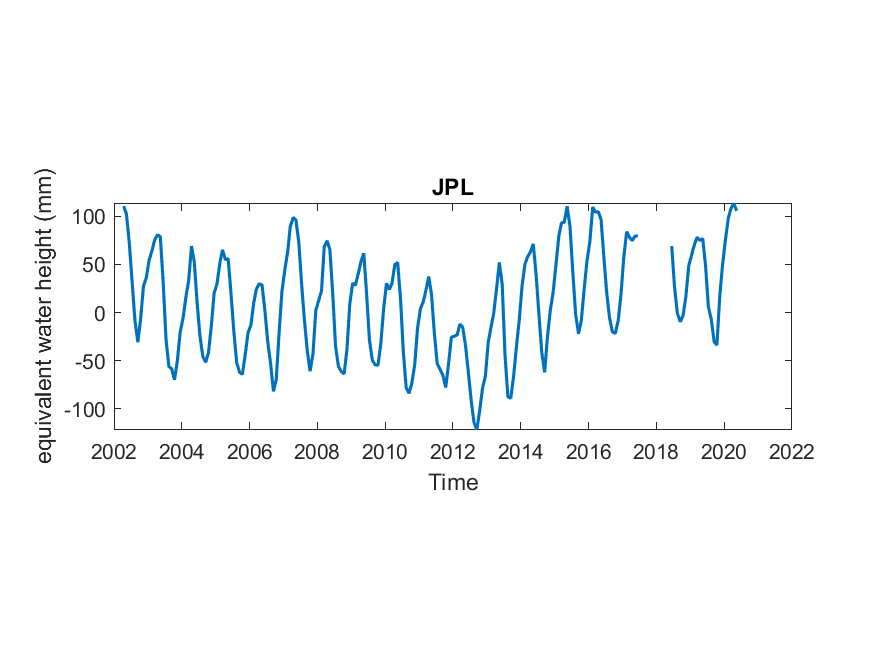
\includegraphics[width=0.8\textwidth]{JPL_TWSA} % Datei in "bilder/" bei LaTeX: eps, bei PDFLaTeX: jpg (o.ä.) 
		\label{fig:JPL}
	\end{minipage}
	\caption{equivalent water height from 4 datasets}
\end{figure}
\\\\
Using the equation \ref{eq:dsdt} we are able to plot the $dS / dt$ for 4 datasets see figure(\ref{fig:dSdt})
\begin{figure}[htbp]\label{fig:dSdt}
	\centering
	\begin{minipage}[t]{0.45\textwidth}
		\centering
		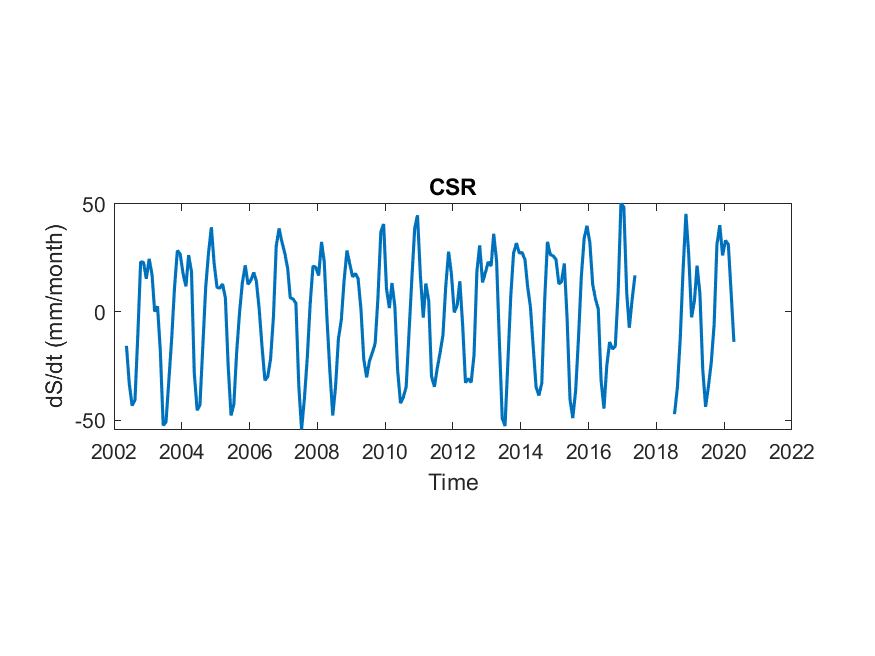
\includegraphics[width=0.8\textwidth]{CSR_dSdt} % Datei in "bilder/" bei LaTeX: eps, bei PDFLaTeX: jpg (o.ä.) 
		\label{fig:CSRdS}
	\end{minipage}
	\begin{minipage}[t]{0.45\textwidth}
		\centering
		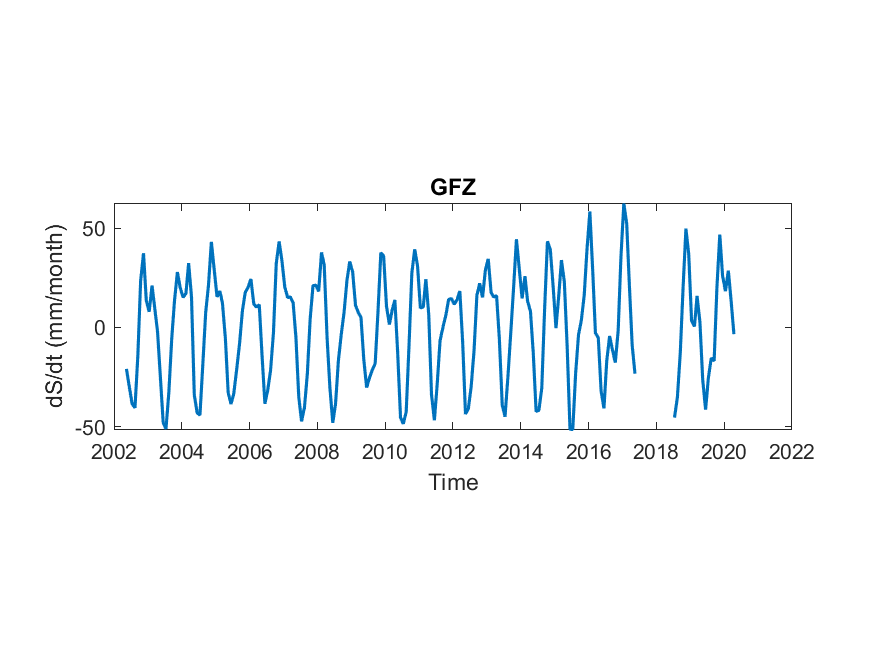
\includegraphics[width=0.8\textwidth]{GFZ_dSdt} % Datei in "bilder/" bei LaTeX: eps, bei PDFLaTeX: jpg (o.ä.) 
		\label{fig:GFZdS}
	\end{minipage}
	\begin{minipage}[t]{0.45\textwidth}
		\centering
		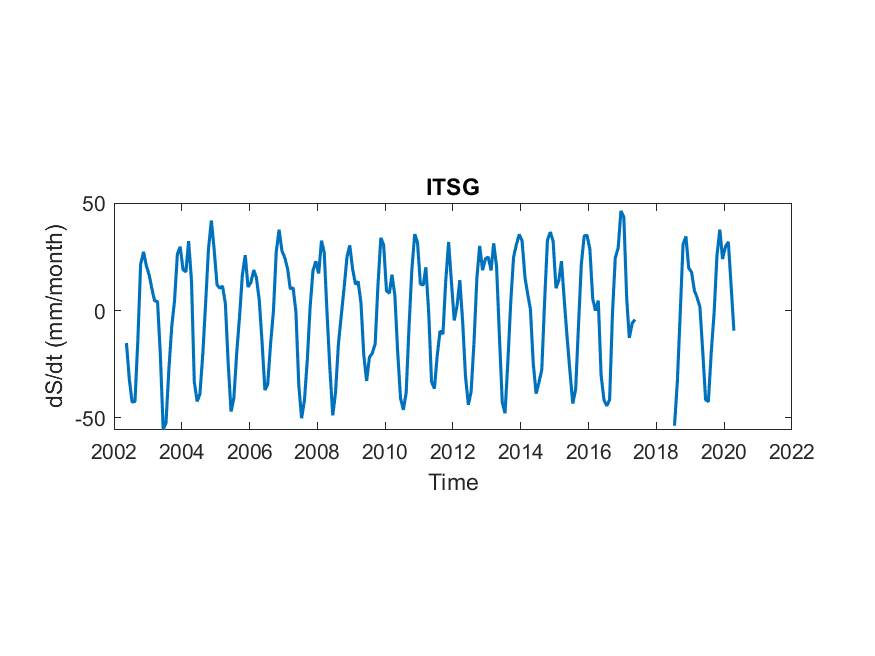
\includegraphics[width=0.8\textwidth]{ITSG_dSdt} % Datei in "bilder/" bei LaTeX: eps, bei PDFLaTeX: jpg (o.ä.) 
		\label{fig:ITSGdS}
	\end{minipage}
	\begin{minipage}[t]{0.45\textwidth}
		\centering
		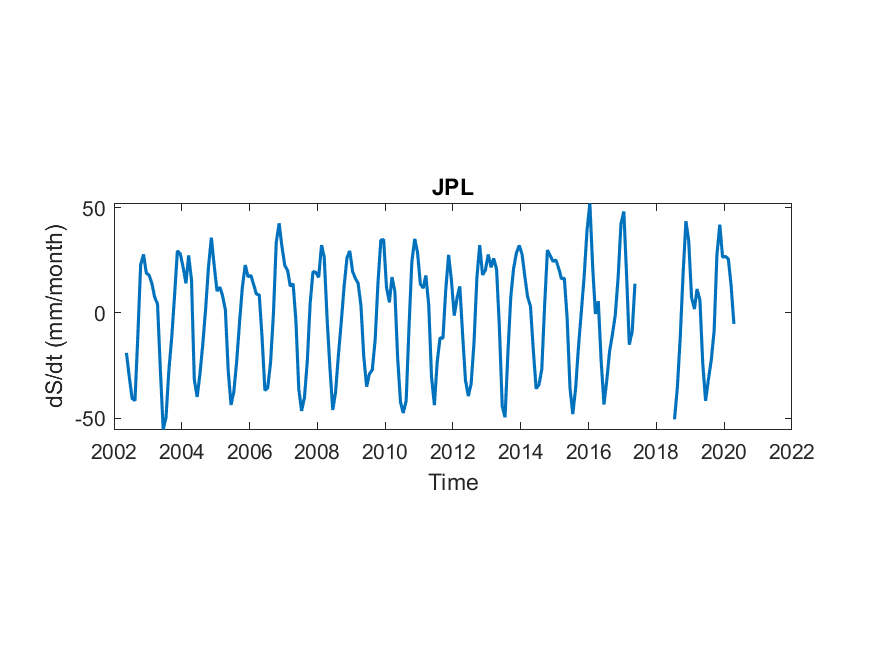
\includegraphics[width=0.8\textwidth]{JPL_dSdt} % Datei in "bilder/" bei LaTeX: eps, bei PDFLaTeX: jpg (o.ä.) 
		\label{fig:JPLdS}
	\end{minipage}
	\caption{$dS / dt$ from 4 datasets}
\end{figure}
\\\\
After that, we can plot one time series with the method mentioned in \ref{section:oneseries}. See figure(\ref{fig:dsdt1})
\begin{figure}[htbp]\label{fig:dsdt1} 
	\centering
	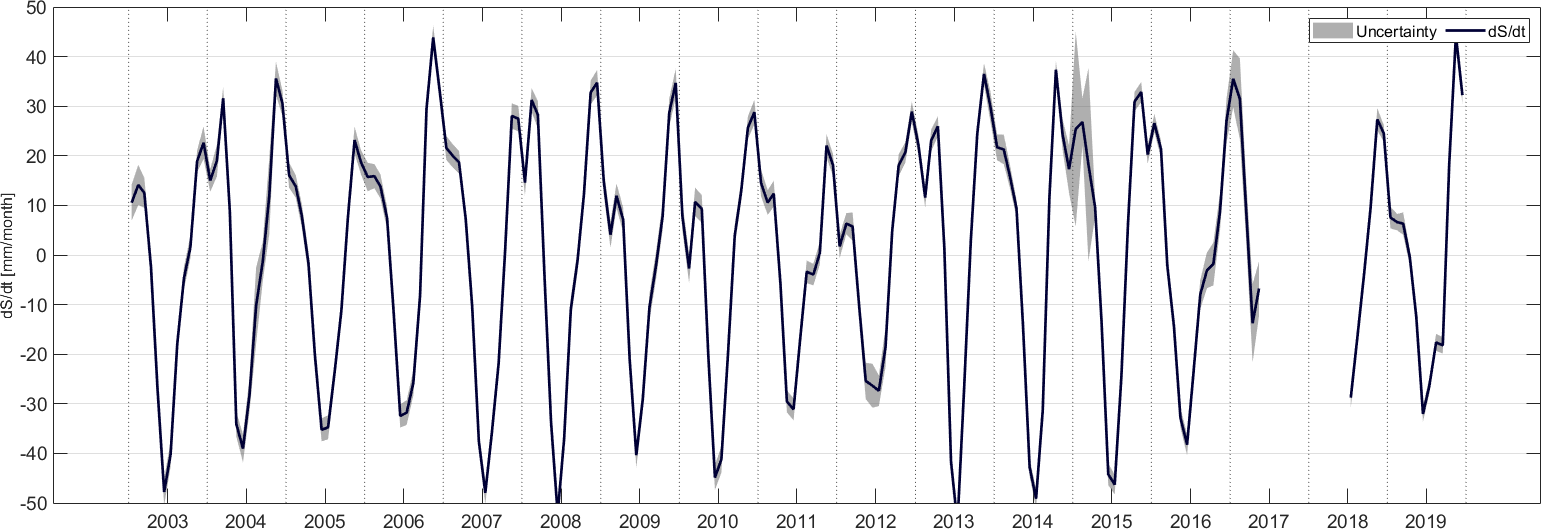
\includegraphics[width=0.7\textwidth]{dSdt} % Datei in "bilder/" bei LaTeX: eps, bei PDFLaTeX: jpg (o.ä.) 
	\caption{$dS/dt$ generated from all datasets} 
	\label{fig:onetimeserie}
\end{figure}
\\\\
In \ref{fig:twsa} we assume that the equivalent water height are stable before 2011. There maybe a small decline between 2010 and 2012 and since 2013 we can see an obvious positive trend. The whole time series then can divide to 3 phases, 